
%(BEGIN_QUESTION)
% Copyright 2012, Tony R. Kuphaldt, released under the Creative Commons Attribution License (v 1.0)
% This means you may do almost anything with this work of mine, so long as you give me proper credit

Skisser kvalitativt hvordan en regulator med kun integralvirkning responderer over tid på følgende endringer i prosessvariabelen:

$$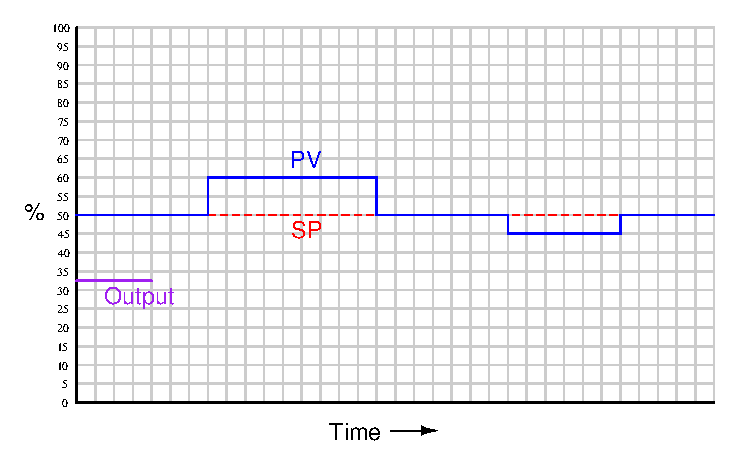
\includegraphics[width=15.5cm]{i01594x01.eps}$$

Anta {\it revers} reguleringsvirkning.

\vskip 20pt \vbox{\hrule \hbox{\strut \vrule{} {\bf Forslag til sokratisk diskusjon} \vrule} \hrule}

\begin{itemize}
\item{} Hvordan ville regulatorresponsen blitt annerledes hvis regulatoren var konfigurert for {\it direkte} virkning i stedet?
\item{} Hvilke faktor(er) avgjør om man skal bruke direkte eller revers reguleringsvirkning?
\item{} Forklar hvorfor det ville være svært uvanlig å se en trend som dette i en reell, fungerende prosess-sløyfe. Hvorfor er denne trenden urealistisk, gitt en fungerende prosess der alle komponenter virker som de skal?
\item{} Gitt at trenden er urealistisk: hvorfor studerer vi den likevel? Med andre ord, hvilken verdi har en slik ``øvings-trend'' for oss?
\end{itemize}

\underbar{file i01594}
%(END_QUESTION)





%(BEGIN_ANSWER)

Regulatorutgangens graf vist her er kun {\it kvalitativ}. Selv om den er tegnet i riktig proporsjon (dvs. alle endringer i utgangen er riktig skalert relativt til hverandre), er selve skalaen vilkårlig og matcher derfor ikke nødvendigvis skalaen i din egen skisse:

$$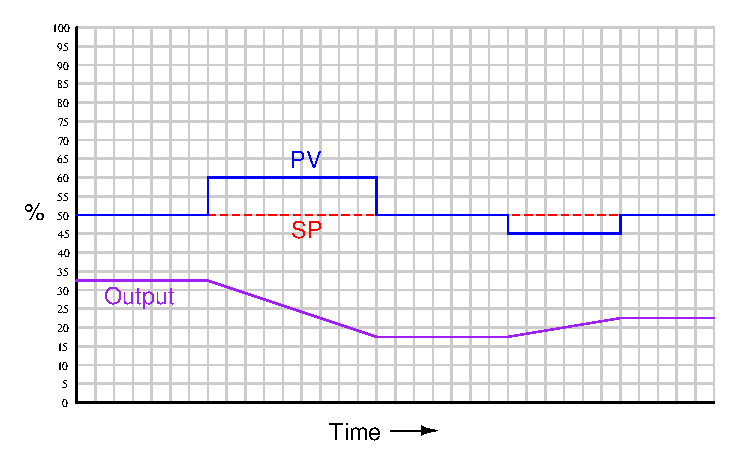
\includegraphics[width=15.5cm]{i01594x02.eps}$$

%(END_ANSWER)





%(BEGIN_NOTES)

{\bf Proporsjonalvirkning er når avvikets størrelse forteller utgangen hvor \underbar{langt} den skal gå.}

\vskip 10pt

{\bf Integralvirkning er når avvikets størrelse forteller utgangen hvor \underbar{raskt} den skal gå.}

\vskip 10pt

{\bf Derivatvirkning er når \underbar{hastigheten} til avviket forteller utgangen hvor \underbar{langt} den skal gå.}

\vskip 10pt


Selv om oppgaven bare ber om en {\it kvalitativ} skisse, er det viktig at studentene er nøye og tegner skissene så proporsjonalt korrekte som mulig. I svaret kan du for eksempel se at første rampeperiode endres med 15\%, mens andre rampeperiode endres med bare 5\%, fordi arealet integrert under første avviksperiode er {\it tre ganger større} enn arealet under andre avviksperiode. Studentenes kvalitative skisser bør vise det samme forholdet 3:1.

En vanlig misforståelse er at mange studenter tegner rampestørrelsen lik avviksstørrelsen. Det er feil, fordi det fullstendig ignorerer {\it tid} som variabel i integrasjon.










\vfil \eject

\noindent
{\bf Oppsummeringsquiz:}

Anta at en student skisserer denne utgangstrenden for å forklare hva en direktevirkende regulator med kun integralvirkning ville gjort som respons på de to ``trinnene'' i prosessvariabelen:

$$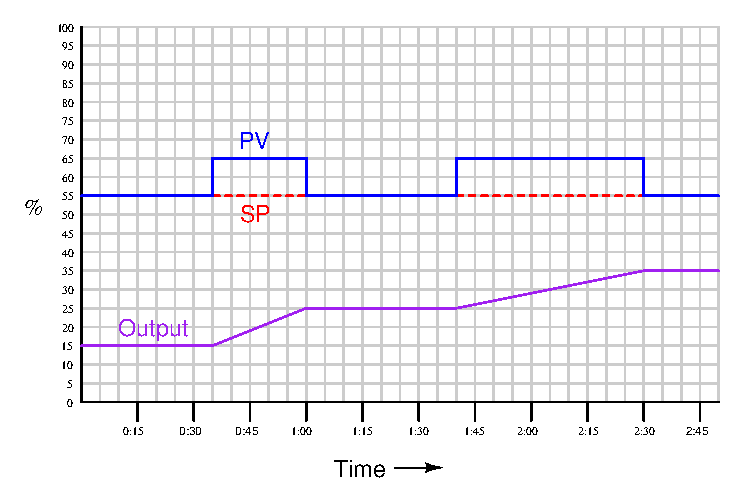
\includegraphics[width=15.5cm]{i01594x03.eps}$$

Dette er {\it ikke} det en virkelig regulator med kun integralvirkning ville gjort. Forklar hva som er feil i studentens skisse av utgangen.

%INDEX% Control, integral: graphing controller response

%(END_NOTES)
